\documentclass[a4paper,12pt]{article}
\usepackage{graphicx}
\usepackage{bm,amssymb}
\usepackage{mathrsfs}
\usepackage[unicode,colorlinks=true,filecolor=blue, menucolor=black, linkcolor=black, citecolor=black,pagebackref=white]{hyperref}
\usepackage[utf8]{inputenc}
\usepackage[russian]{babel}
\usepackage{amsmath}
\usepackage{caption}
\usepackage[left=2cm,right=2cm, top=2cm,bottom=2cm,bindingoffset=0cm]{geometry}
\begin{document}
\title{Семинар по теме: <<Метод стационарной фазы>>}
\maketitle


Часто в приложениях встречаются определённые осциллирующие интегралы
типа: 
\[
\int_{a}^{b}f(x)e^{i\lambda S(x)}dx
\]
при $\lambda\to+\infty$. В нулевом приближении по большому $\lambda$ интеграл зануляется. Интерес представляет нахождение поправки.  

\noindent
Для начала рассмотрим случай, когда $S^{'}(x)\ne0$ $\forall x\in [a;b]$. Имеем:
$$
\int_{a}^{b}e^{i\lambda S(x)}f(x)=\frac{1}{i\lambda}\left(\frac{1}{S^{'}(b)}f(b)e^{i\lambda S(b)}-\frac{1}{S^{'}(a)}f(a)e^{i\lambda S(a)}\right)-\frac{1}{i\lambda}\int_{a}^{b}e^{i\lambda S(x)}\frac{f^{'}(x)}{S^{'}(x)}dx
$$
Последующим интегрированием по частям легко показывается, что в главном приближении по $\lambda^{-1}$ ответ даётся внеинтегральным членом.

\noindent
Этот метод работает, когда у фазы (функции $S(x)$) нет стационарной точки на области интегрирования. Рассмотрим случай, когда она есть и одна на всей области интегрирования:
$$
e^{i\lambda S(x_0)}\int_{a}^{b}e^{i\lambda( S(x)-S(x_0))}f(x)dx=e^{i\lambda S(x_0)}\int_{x^{-1}(a)}^{x^{-1}(b)}g(t)e^{i\lambda t^2}dt
$$
Здесь была произведена замена $\sqrt{S(x)-S(x_0)}=t$. Строго говоря, так можно делать только в том случае, когда $S^{''}(x_0)>0$. Однако, другой случай разбирается полностью аналогично (можете сами проделать это в качестве упражнения), так что мы получим ответ в предположении $S^{''}(x_0)>0$, а затем заменим $S^{''}(x_0)$ на $|S^{''}(x_0)|$. 

\noindent
Последний интеграл равен:
$$
\int_{c}^{d}g(t)e^{i\lambda t^2}dt\approx g(0)\sqrt{\frac{\pi}{2\lambda}}e^{i\pi/4}
$$
Это легко получить, заметив, что из-за быстрых осцилляций интеграл набирается вблизи нуля и разложив $g(t)$ в ряд Тейлора. Кроме того, были использованы следующие интегралы с семинара 4:
\[
\int_{-\infty}^{\infty}\cos(\alpha x^{2})dx=\int_{-\infty}^{\infty}\sin(\alpha x^{2})dx=\sqrt{\frac{\pi}{2\alpha}}
\]
Далее, вспоминая определение функции $g$, получаем, что 
$$
\int_{a}^{b}f(x)e^{i\lambda S(x)}dx=f(x_0)\sqrt{\frac{2\pi}{\lambda |S^{''}(x_0)|}}e^{i\lambda S(x_0)}e^{i\pi/4}
$$
Это и есть то, как работает метод стационарной фазы.


\paragraph{Критерии применимости}

Выше рассматривалась фаза $\lambda S(x)$. В этом случае критерием применимости метода стационарной фазы является $\lambda\gg 1$. Однако, аналогично методу перевала, можно рассмотреть фазу $S(x)$, не cодержащую явно большой параметр. Тогда критерий применимости можно получить из следующих рассуждений: интеграл
от разложенной функции набирается в малой окрестности стационарной
точки шириной $|x-x_{0}|\sim\frac{1}{\sqrt{|S^{\prime\prime}(x_{0})|}}$
(там, где фаза $S(x)$ изменяется на число порядка 1). Тогда пренебрежение
следующими членами разложения в ряд Тейлора верно при выполнении следующих
условий: 
\[
\begin{cases}
|S^{(3)}(x_{0})(x-x_{0})^{3}| & \ll|S^{\prime\prime}(x_{0})(x-x_{0})^{2}|\\
|S^{(4)}(x_{0})(x-x_{0})^{4}| & \ll|S^{\prime\prime}(x_{0})(x-x_{0})^{2}|
\end{cases}\Rightarrow\begin{cases}
|S^{(3)}(x_{0})| & \ll|S^{\prime\prime}(x_{0})|^{3/2}\\
|S^{(4)}(x_{0})| & \ll|S^{\prime\prime}(x_{0})|^{2}
\end{cases}
\]



\subsection*{Задача 1 (функция Эйри)}

В качестве примера разберем поведение функции Эйри (Airy) при $x\to-\infty$:

\[
{\rm Ai}\left(x\right)=\frac{1}{\pi}\int_{0}^{\infty}\cos\left(\frac{t^{3}}{3}+xt\right)dt
\]



\subsubsection*{Решение}

Найдем стационарные точки фазы:
\[
f^{\prime}(t)=t^{2}+x=0\Rightarrow t_{1,2}=\pm|x|^{1/2}
\]

\noindent
Только одна стационарная точка $t_{1}=\sqrt{-x}$ попадает в отрезок
интегрирования, и необходимо рассматривать вклад только от ее окрестности.
Для поведения фазы в окрестности этой точки можно записать:
\[
f^{\prime\prime}(t)=2t\Rightarrow f^{\prime\prime}(t_{1})=2|x|^{1/2}
\]
\[
f(t)\approx-\frac{2}{3}|x|^{3/2}+|x|^{1/2}(t-|x|^{1/2})^{2}
\]

\noindent
Поэтому вклад в интеграл от окрестности стационарной точки записывается
как:
\begin{multline*}
{\rm Ai}(x)\approx\frac{1}{\pi}\int_{-\infty}^{\infty}\cos\left(-\frac{2}{3}|x|^{3/2}+|x|^{1/2}(t-|x|^{1/2})^{2}\right)\cdot dt=\\
=\frac{1}{\pi}\int_{-\infty}^{\infty}\left(\cos\left(\frac{2}{3}|x|^{3/2}\right)\cos\left(|x|^{1/2}(t-|x|^{1/2})^{2}\right)+\sin\left(\frac{2}{3}|x|^{3/2}\right)\sin\left(|x|^{1/2}(t-|x|^{1/2})^{2}\right)\right)dt=\\
=\frac{1}{\pi}\left(\cos\left(\frac{2}{3}|x|^{3/2}\right)+\sin\left(\frac{2}{3}|x|^{3/2}\right)\right)\sqrt{\frac{\pi}{2|x|^{1/2}}}=\frac{1}{\sqrt{\pi}|x|^{1/4}}\sin\left(\frac{2}{3}|x|^{3/2}+\frac{\pi}{4}\right)
\end{multline*}


\begin{figure}[h]
\caption{Функция Эйри ${\rm Ai}(x)$ при $x<0$ и её асимптотика}
\centering
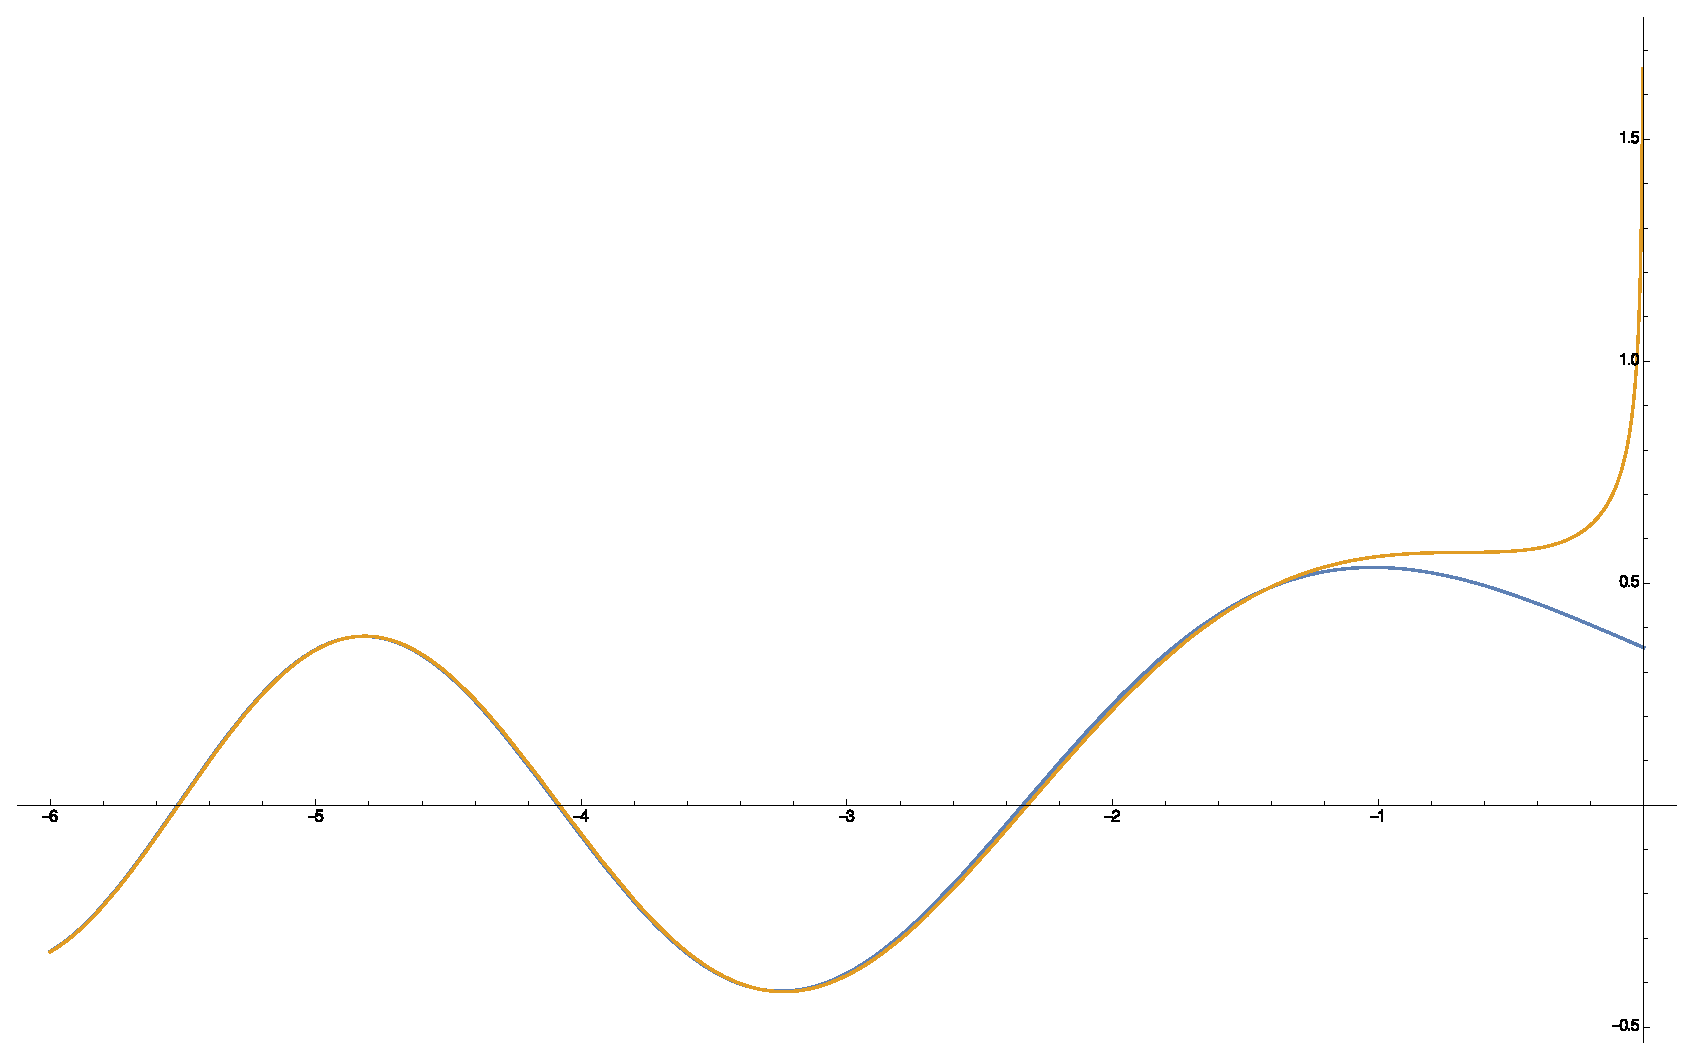
\includegraphics[width=0.65\columnwidth]{airy.eps}
\end{figure}



\subsection*{Задача 2 (функция Бесселя)}

Разберем поведение функции Бесселя при $x\to\infty$:
\[
J_{0}(x)=\frac{1}{\pi}\int_{0}^{\pi}\cos(x\sin t)dt
\]



\subsubsection*{Решение}

Стационарные точки фазы даются условием:
\[
f^{\prime}(t)=x\cos t=0\Rightarrow t_{n}=\frac{\pi}{2}+\pi n
\]

\noindent
В отрезок интегрирования попадает одна стационарная точка $t_{0}$;
поведение функции определяется вкладом в интеграл лишь от окрестности
этой точки. Имеем:
\[
f^{\prime\prime}(t)=-x\sin t\Rightarrow f^{\prime\prime}(t_{0})=-x
\]


\[
f(t)\approx x-\frac{1}{2}x\left(t-\frac{\pi}{2}\right)^{2}
\]

\noindent
поэтому для оценки асимптотики функции Бесселя получаем:
\begin{multline*}
J_{0}(x)\approx\frac{1}{\pi}\int_{-\infty}^{\infty}\cos\left(x-\frac{1}{2}x\left(t-\frac{\pi}{2}\right)^{2}\right)dt=\\
=\frac{1}{\pi}\int_{-\infty}^{\infty}\left(\cos x\cdot\cos\left(\frac{1}{2}x\left(t-\frac{\pi}{2}\right)^{2}\right)+\sin x\cdot\sin\left(\frac{1}{2}x\left(t-\frac{\pi}{2}\right)^{2}\right)\right)dt=\\
=\frac{1}{\pi}(\cos x+\sin x)\sqrt{\frac{2\pi}{2x}}=\sqrt{\frac{2}{\pi x}}\sin\left(x+\frac{\pi}{4}\right)
\end{multline*}


\begin{figure}[h]
\caption{Функция Бесселя $J_{0}(x)$ и её асимптотика}
\centering
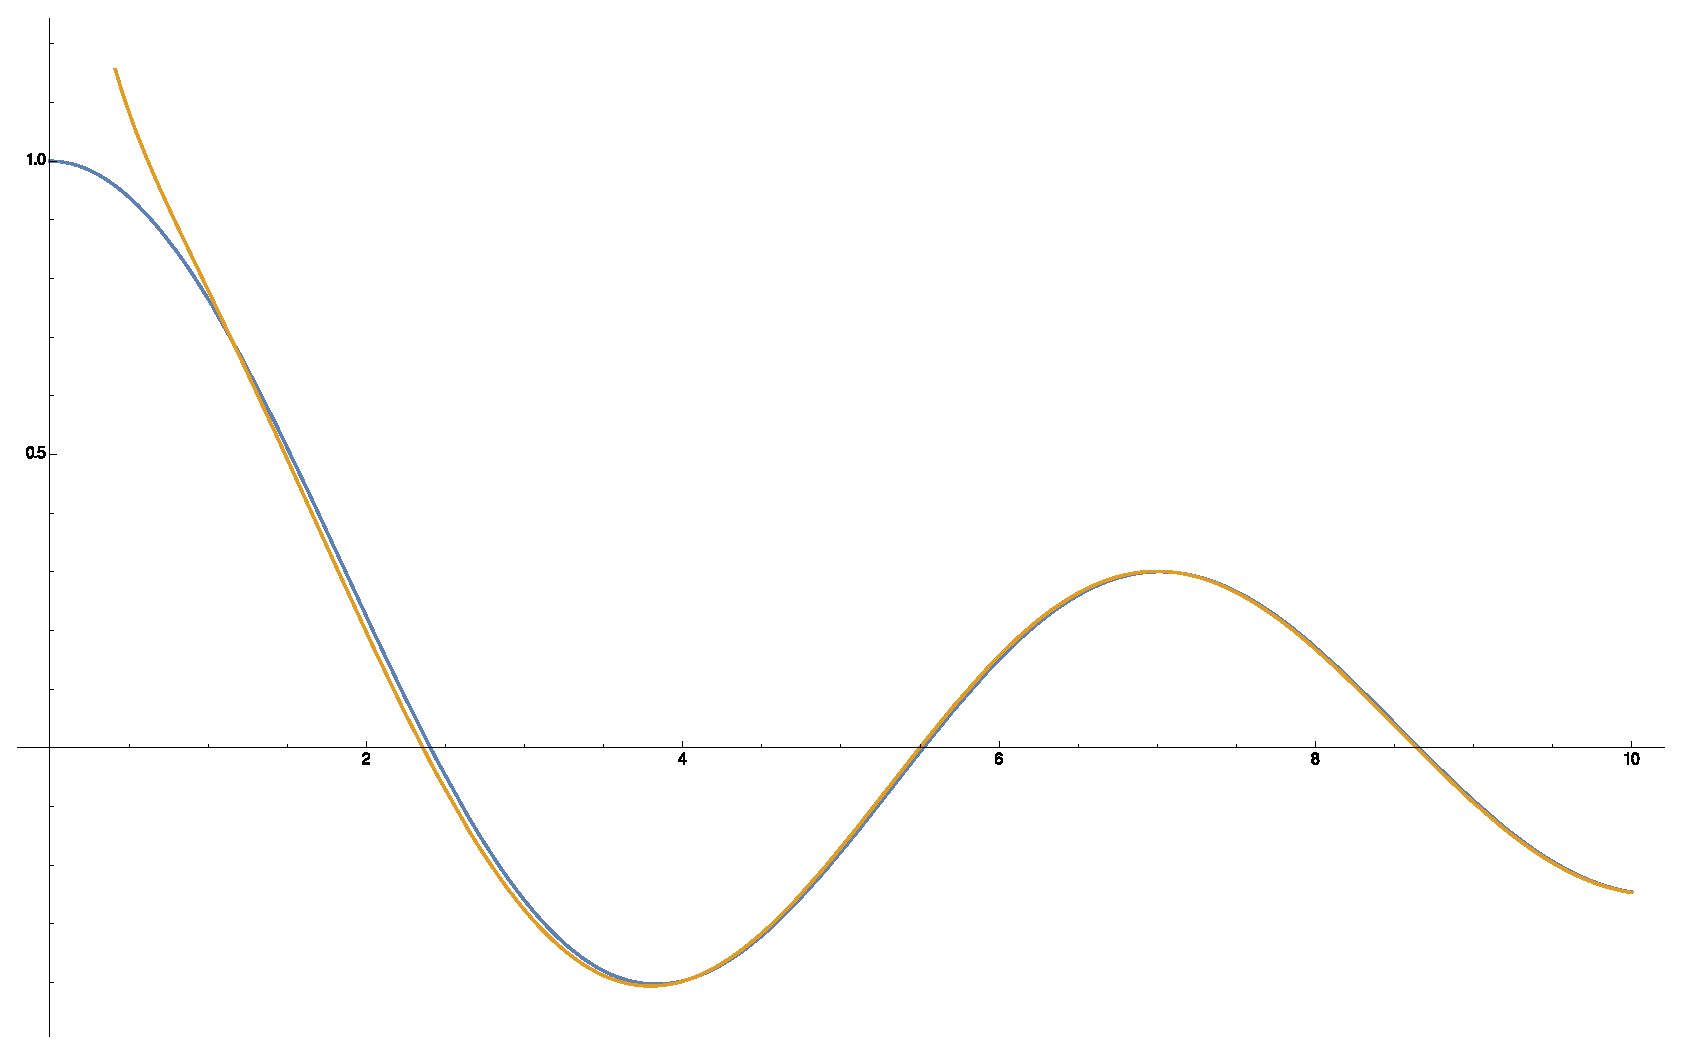
\includegraphics[width=0.65\columnwidth]{besselj.eps}
\end{figure}


\subsection*{Асимптотические разложения}

Практически во всех задачах мы сталкивались с асимптотическими разложениями
в том или ином виде; и каждый раз мы находили первые несколько членов
этого самого разложения. Поясним теперь, что из себя представляют
эти самые разложения. Пусть имеется функция $f(x)$ и последовательность
функций $\varphi_{k}(x)$. Мы будем говорить, что функции $\varphi_{k}(x)$
представляют собой асимптотическое разложение функции $f(x)$ в окрестности
точки $x_{0}$ (может быть и бесконечно удалённой), и писать
\[
f(x)\sim\sum_{k=0}^{\infty}\varphi_{k}(x),\quad x\to x_{0}
\]

\noindent
если, во-первых, каждый следующий член этого ряда меньше предыдущего:
\[
\varphi_{k}(x)\gg\varphi_{k+1}(x)\Leftrightarrow\varphi_{k+1}(x)=\overline{o}(\varphi_{k}(x)),\quad x\to x_{0}
\]

\noindent
а во-вторых, функцию можно приблизить суммированием конечного члена
этого ряда:
\[
f(x)=\sum_{k=0}^{N}\varphi_{k}(x)+\underline{O}(\varphi_{N+1}(x)),\quad x\to x_{0}
\]



\paragraph{Замечание}

Тут уместо сделать несколько замечаний. Во-первых, разложения в ряд
Тейлора представляют собой пример асимптотических разложений с функциями
$\varphi_{k}(x)=\frac{f^{(k)}(x_{0})}{k!}(x-x_{0})^{k}$. А во-вторых,
как правило в приложениях, асимптотические ряды формально непригодны
для подсчёта значений функции в любой конкретной точке по той причине,
что они часто \textbf{расходятся}. Это, тем не менее, не мешает их активно
использовать для асимптотического анализа и приближенных оценок, как
мы поступали с задачами ранее. В частности, так называемый метод диаграм
Фейнмана представляет собой пример асимптотических разложений.


\subsection*{Задача 3 (функция Макдональда)}

Найти асиптотическое разложение для интеграла при $a\to\infty$ 
\[
I(a)=\int_{0}^{\infty}\frac{e^{-x}}{\sqrt{x(x+\alpha)}}dx
\]



\subsubsection*{Решение}

Асимптотический ряд можно просто получить, раскладывая корень по малости
$\frac{x}{\alpha}$. Имеем:
\[
I\left(a\right)=\int_{0}^{\infty}\frac{e^{-x}}{\sqrt{x(x+\alpha)}}dx=\frac{1}{\sqrt{\alpha}}\int_{0}^{\infty}\frac{e^{-x}}{\sqrt{x}}\left(1+\frac{x}{\alpha}\right)^{-1/2}dx=\frac{1}{\sqrt{\alpha}}\int_{0}^{\infty}\frac{e^{-x}}{\sqrt{x}}\cdot\sum_{k=0}^{\infty}C_{-1/2}^{k}\left(\frac{x}{\alpha}\right)^{k}dx
\]

\noindent
Тут $C_{\alpha}^{k}$ при нецелых $\alpha$ - обобщенный биномиальный
коэффициент, определяемый как:
\[
C_{\alpha}^{k}=\frac{\alpha(\alpha-1)\dots(\alpha-k+1)}{k!}=\frac{\Gamma(\alpha+1)}{\Gamma(\alpha-k+1)\Gamma(k+1)}
\]

\noindent
В случае $\alpha=-\frac{1}{2}$ это можно переписать:
\[
C_{-1/2}^{k}
=
\frac{   \left(-\frac{1}{2}\right)  \left(-\frac{3}{2}\right)...\left(-k+\frac{1}{2}\right)}{k!} = \frac{(-1)^{k}}{2^{k}}\cdot\frac{(2k-1)!!}{k!}
\]

\noindent
Дальше можно поменять местами сумму и интеграл; каждый из полученных
интегралов представляет собой просто интеграл Эйлера; получаем:
\begin{multline*}
I(a)\sim\frac{1}{\sqrt{\alpha}}\sum_{k=0}^{\infty}\frac{1}{\alpha^{k}}C_{-1/2}^{k}\int_{0}^{\infty}e^{-x}x^{k-\frac{1}{2}}dx=\sum_{k=0}^{\infty}\frac{1}{\alpha^{k+1/2}}C_{-1/2}^{k}\Gamma\left(k+\frac{1}{2}\right)=\\
=\sum_{k=0}^{\infty}\frac{1}{\alpha^{k+1/2}}\cdot\frac{(-1)^{k}}{2^{k}}\cdot\frac{\left(2k-1\right)!!}{k!}\frac{\left(2k-1\right)!!}{2^{k}}\sqrt{\pi}=\sum_{k=0}^{\infty}\frac{1}{\alpha^{k+1/2}}\cdot\frac{(-1)^{k}((2k-1)!!)^{2}\sqrt{\pi}}{2^{2k}k!}
\end{multline*}

\noindent
тут мы воспользовались тем, что $\Gamma\left(k+\frac{1}{2}\right)=\left(k-\frac{1}{2}\right)\cdot\left(k-\frac{3}{2}\right)\cdot\dots\cdot\frac{1}{2}\Gamma\left(\frac{1}{2}\right)=\frac{(2k-1)!!}{2^{k}}\sqrt{\pi}$.
Для первых нескольких членов разложения имеем:
\[
I(a)=\sqrt{\frac{\pi}{\alpha}}\left(1-\frac{1}{4\alpha}+\frac{9}{32\alpha^{2}}+O\left(\frac{1}{\alpha^{3}}\right)\right)
\]

\noindent
Уместно заметить, что полученный асимптотический ряд расходится для любого значения $\alpha$.
\textit{Кроме того, отметим для справки, что точный ответ
выражается через модифицированную функцию Бесселя - так называемую
функцию Макдональда $I(a)=e^{\alpha/2}K_{0}(\alpha/2)$.}

\begin{figure}[h]
\caption{Точное значение интеграла и первые два члена асимптотического разложения}
\centering
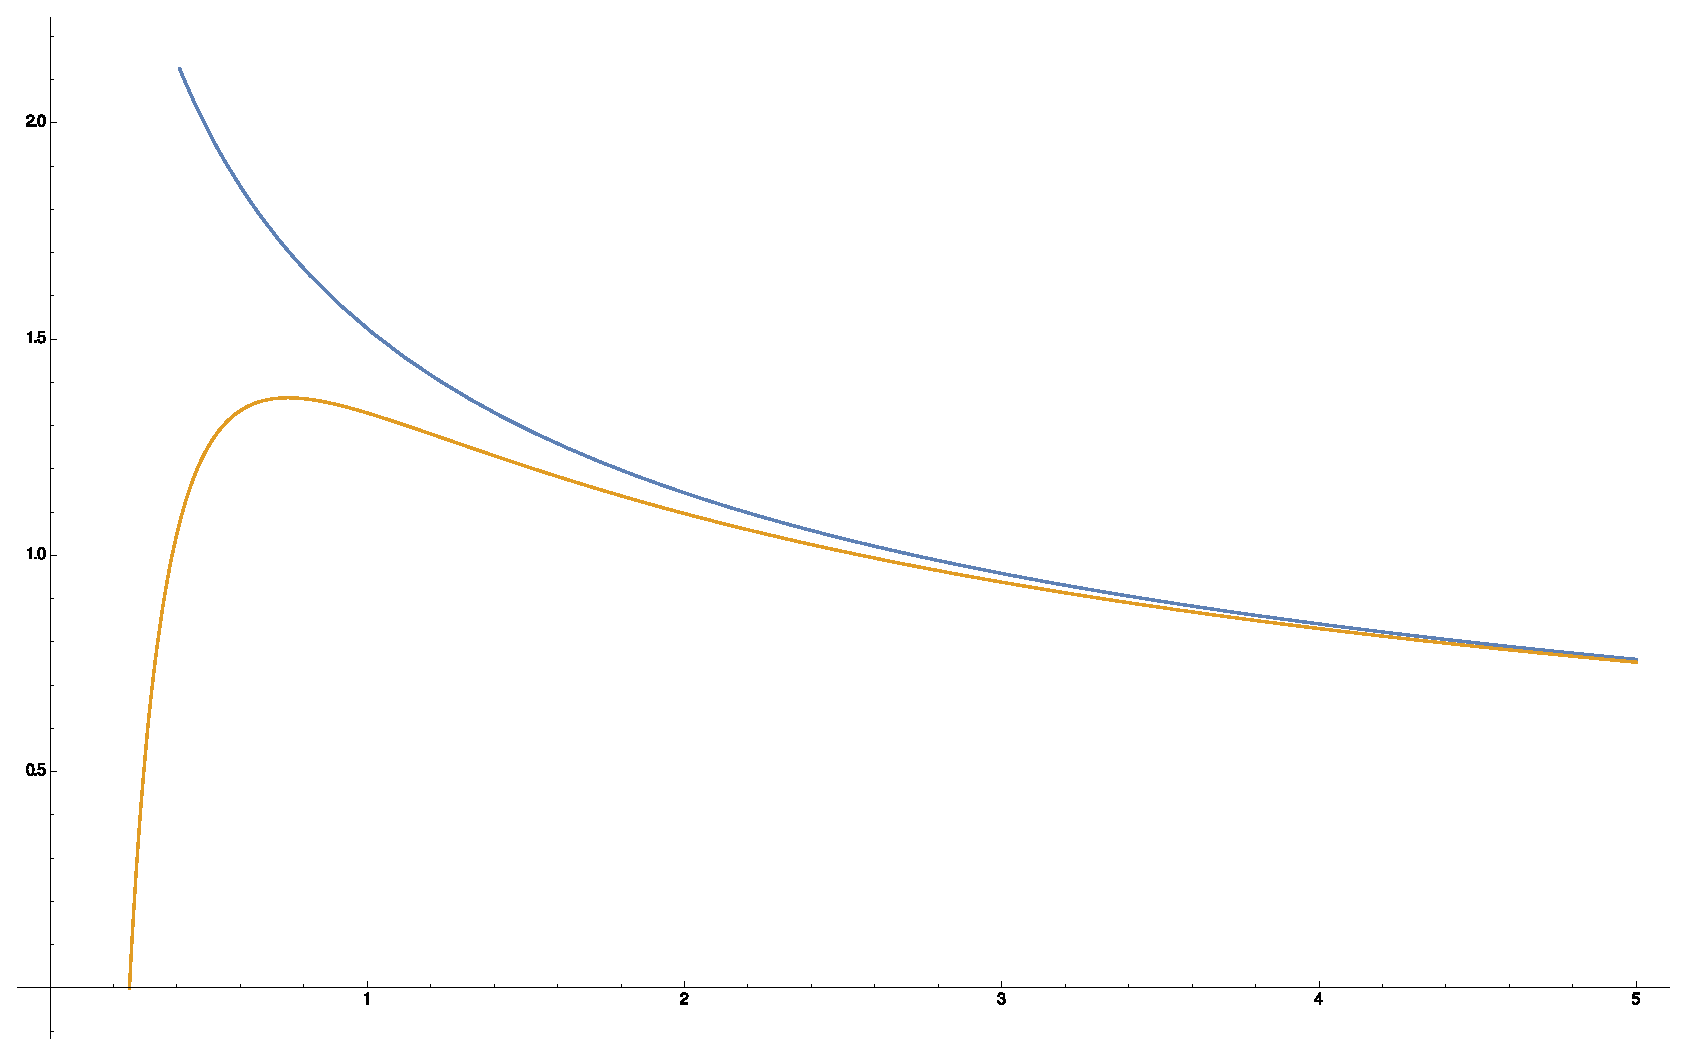
\includegraphics[width=0.65\columnwidth]{besselk.eps}
\end{figure}



\subsection*{Задача 4 (интегральный синус)}

Найдём полное асимптотическое разложение интегрального синуса при
$x\to\infty$:
\[
{\rm Si}(x)=\int_{0}^{x}\frac{\sin t}{t}dt
\]



\subsubsection*{Решение}

Перепишем выражение следующим образом, используя интеграл Дирихле:
\[
{\rm Si}(x)=\frac{\pi}{2}-\int_{x}^{\infty}\frac{\sin t}{t}dt
\]

\noindent
Можно получить асимптотический ряд, просто интегрируя по частям:
\[
{\rm Si}(x)=\frac{\pi}{2}-\int_{x}^{\infty}\frac{\sin t}{t}dt=\frac{\pi}{2}-\frac{\cos x}{x}+\int_{x}^{\infty}\frac{\cos t}{t^{2}}dt=\frac{\pi}{2}-\frac{\cos x}{x}-\frac{\sin x}{x^{2}}+2\int_{x}^{\infty}\frac{\sin t}{t^{3}}dt
\]

\noindent
В общем виде мы получаем следующую сумму:
\[
{\rm Si}(x)=\frac{\pi}{2}-\cos x\sum_{k=0}^{\infty}\frac{(-1)^{k}(2k)!}{x^{2k+1}}-\sin x\sum_{k=0}^{\infty}\frac{(-1)^{k}(2k-1)!}{x^{2k}}
\]

\noindent
Первые несколько членов ряда дают:
\[
{\rm Si}(x)=\frac{\pi}{2}-\frac{\cos x}{x}-\frac{\sin x}{x^{2}}+2\frac{\cos x}{x^{3}}+O\left(\frac{1}{x^{4}}\right)
\]

\noindent
Отметим, что, как и в предыдущем случае, полученные ряды также расходятся.

\begin{figure}[h]
\caption{Интегральный синус ${\rm Si}(x)$ и первое приближение}
\centering
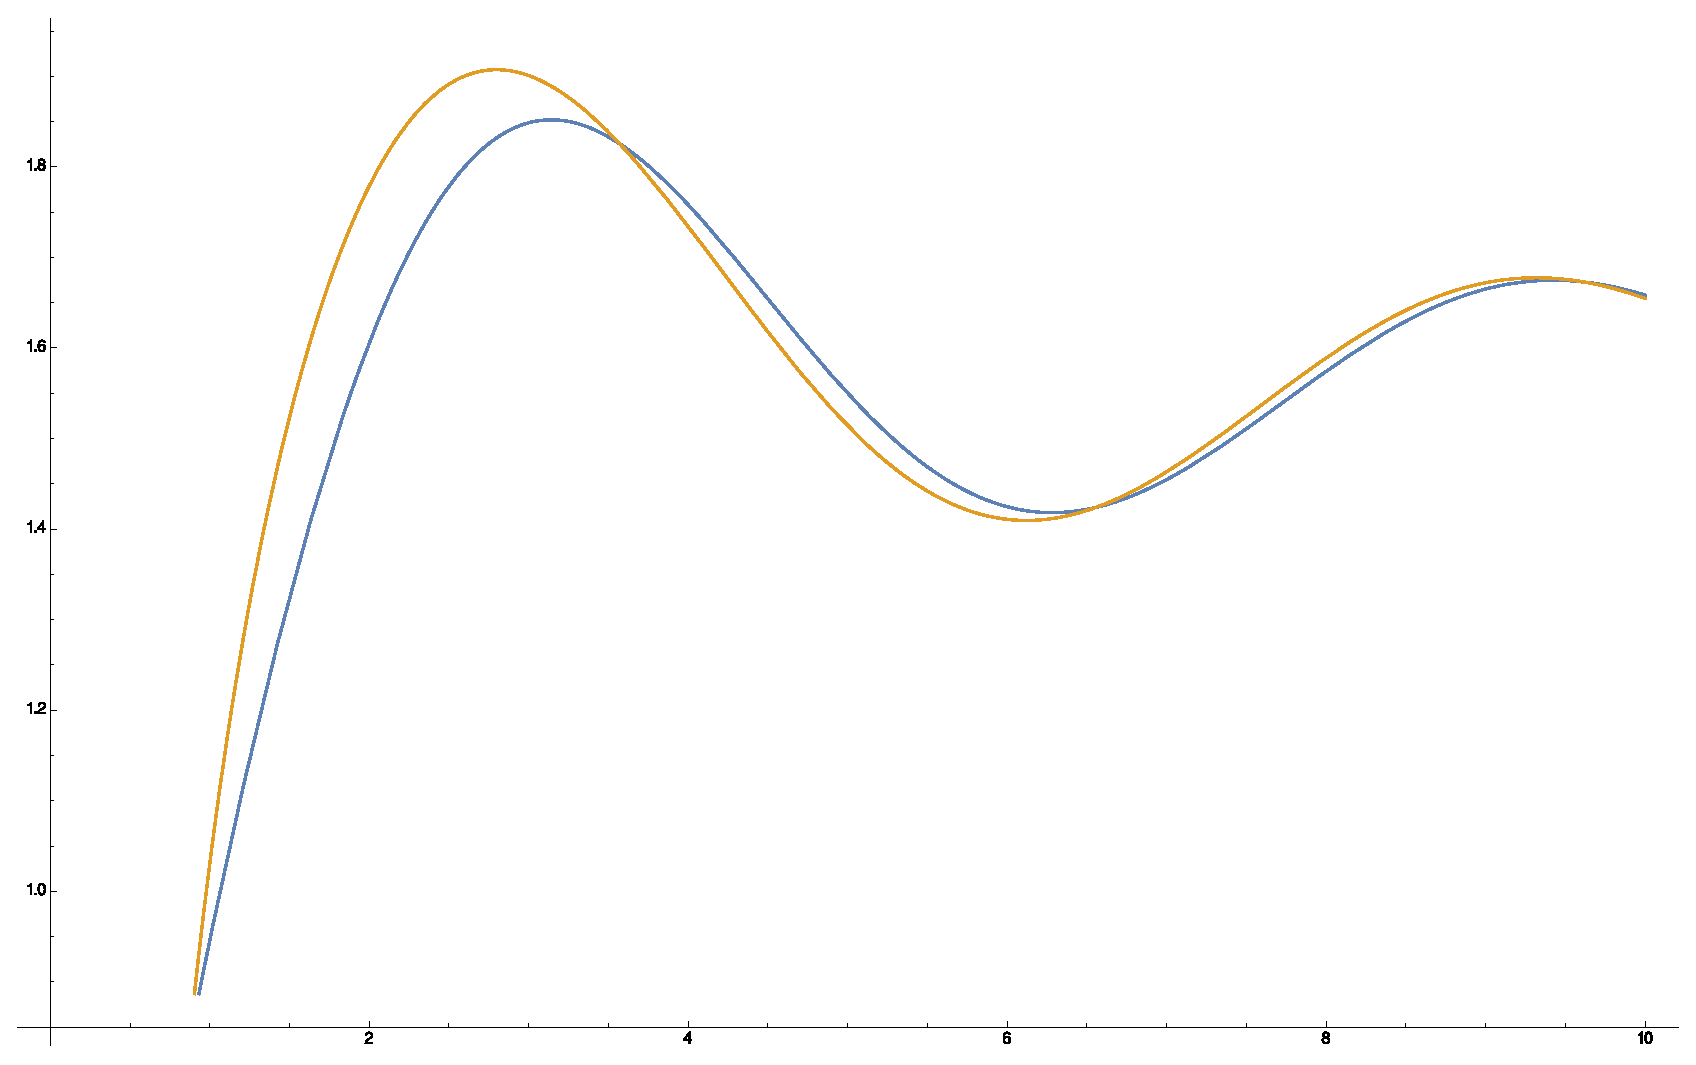
\includegraphics[width=0.65\columnwidth]{sinintegral.eps}
\end{figure}


\subsection*{Задача 5}

Покажем, что функция 
\[
\delta_{\omega}(x)=\frac{1}{\pi}\cdot\frac{\sin^{2}(\omega x)}{\omega x^{2}}
\]

\noindent
при $\omega\to\infty$ представляет собой $\delta$-функцию Дирака.


\subsubsection*{Решение}

Область, в которой функция существенно отлична от нуля, имеет ширину
$\left|x\right|\sim\frac{1}{\omega}$, и при $\omega\to\infty$ она
сужается:
\[
\lim_{\omega\to\infty}\delta_{\omega}(x\neq0)=0
\]

\noindent
поэтому при рассмотрении интеграла вида $I=\int\delta_{\omega}(x)f(x)dx$
при $\omega\to\infty$ поведение определяется окрестностью нуля (область
интегрирования должна содержать ноль, а функция $f\left(x\right)$
не должна иметь сингулярностей в нуле). Получаем:
\[
I\approx\int_{-\infty}^{\infty}\delta_{\omega}(x)f(0)dx=f(0)\frac{1}{\pi}\int_{-\infty}^{\infty}\frac{\sin^{2}\omega x}{\omega x^{2}}dx=f(0)
\]

\noindent
Это и доказывает нужное утверждение:

\[
\lim_{\omega\to\infty}\int_{-\infty}^{\infty}\delta_{\omega}(x)f(x)dx=f(0)\Rightarrow\lim_{\omega\to\infty}\delta_{\omega}(x)=\delta(x)
\]


\subsection*{Задачи для домашнего решения}

\noindent \textbf{Упражнение 1}

\noindent Вычислите значение функции Эйри в $x=0$:

$$
\mathrm{Ai}(x)	=\frac{1}{\pi}\int_{0}^{\infty}dt\cos(\frac{t^{3}}{3}+tx)
$$

\vspace{15pt}
\noindent \textbf{Упражнение 2}

\noindent Приближенно вычислите интеграл при $x\rightarrow+\infty$
$$
I(x)	=\int_{0}^{\infty}\cos(x(t^{2}-t^{4}))dt
$$

\vspace{15pt}
\noindent \textbf{Упражнение 3}

\noindent Получите разложение интегрального косинуса

$$
\mathrm{Ci}(x)	=-\int_{x}^{\infty}\frac{\cos t}{t}dt
$$
\noindent в асимптотический ряд при $x\rightarrow+\infty$.

\vspace{15pt}
\noindent \textbf{Упражнение 4}

\noindent Получите разложение неполной гамма-функции
$$
\Gamma(x,s)	=\int_{x}^{\infty}t^{s-1}e^{-t}dt
$$
\noindent в асимптотический ряд при $x\rightarrow+\infty$ и $s\sim 1$.

\vspace{15pt}
\noindent \textbf{Задача 1}

\noindent Вычислите асимптотику функции Бесселя $n$-ого порядка при $x\gg n$:
$$
J_{n}(x)	=\frac{1}{\pi}\int_{0}^{\pi}\cos(nt-x\sin t)dt.
$$
\noindent Вычислите асимптотику при $x\ll n$. На основе двух асимптотик постройте график функции Бесселя (нужно сшить асимптотики при $x\sim n$).

\vspace{15pt}
\noindent \textbf{Задача 2}

\noindent Приближенно вычислите интеграл
$$
I(x)	=\int_{\pi/2}^{3\pi/2}\sin^{2}t\cos(x\cos t)dt
$$
\noindent при $x\rightarrow+\infty$.
\end{document}
